\chapter{Wstęp}
\label{cha:pierwszyDokument}


Pierwsze obrazy wideo powstały już na początku XX wieku i opierały się na mechanicznie obracających się dyskach. Technologia ta istniała głownie w sferze badań akademickich i nie zdominowała rynku. Dopiero z wprowadzeniem cathode-ray tube (CRT) wraz z telewizją analogową, wideo zaczęło być wykorzystywane komercyjnie. Z czasem rozwój technologii pozwolił na wprowadzenie telewizji cyfrowej, która zapewniała wyższą jakość obrazu oraz lepsze wykorzystanie zasobów. Wideo razem z audio okazały się również znakomitym środkiem wymiany informacji. Stały się coraz częściej wykorzystywane do komunikacji w czasie rzeczywistym zastępując tradycyjne połączenie telefoniczne w biznesie oraz dla zwykłych użytkowników. Również rozwój na rynku telefonów wspomógł powszechność wideo. W momencie kiedy praktycznie każdy aparat zaczął posiadać kamerę, wideo zaczęło konkurować ze zdjęciami jako metoda na utrwalenia chwili. Codziennie tak rejestrowane obrazy są przekazywane do rodziny, znajomych oddalonych o tysiące kilometrów. Kolejnym przykładem kiedy wideo zastępuje tradycyjne formy przekazu są blogi internetowe do tej pory prowadzone na zasadzie artykułów/postów, teraz zaczęły wykorzystywać wideo jako metodę przekazu informacji.

Dzięki coraz większym przepustowością i szerokiemu dostępowi do Internetu w najnowszych czasach wykreował się jeszcze inny trend sprawiający że obrazy wideo są bardziej popularne. Mowa tu o platformach streamingowych takich jak - YouTube, Netflix czy HBOgo. Pozwalają one użytkownikom na oglądanie od krótkich filmików, przez seriale, po pełnometrażowe filmy nawet w rozdzielczościach 4k. Przewidywane jest, że do 2022, aż 82 procent całego ruchu IP, to będzie wideo \cite{prediction}. \par

%.Jako kolejny kierunek rozwoju wideo można potraktować powstałe w ostatnich latach platformy, typu Youtube, netflix czy HBOgo, pozwalające użytkownikom na streamowanie od krótkich %filmików, przez seriale, po pełnometrażowe filmy nawet w rozdzielczościach 4k. \par

Wszystkie wymienione wyżej aspekty sprawiły, że wideo stało się codziennością w życiu większości ludzi.\par

Na obecnym etapie rozwoju technologii, oczekiwania odbiorcy co do jakości otrzymywanego wideo znacznie wzrosły. Na drugiej szali pozostają ograniczenia dotyczące medium i optymalnego wykorzystania zasobów po stronie klienta i serwera(?dostawcy?). Odnosząc się do powyższego istotną kwestią staje się monitorowanie jakości transmitowanego wideo i dostosowywanie go do potrzeb użytkownika. Jednak problem w ocenie jakości wideo jest tu o tyle trudny, że dotychczas najbardziej wiarygodnym wskaźnikiem jest tu opinia ludzka,  trudna do powiązania z mierzalnymi technicznymi, parametrami wideo. W niniejszej Pracy zostanie przedstawiony algorytm pozwalający na bardziej zautomatyzowaną ocenę jakości wideo w oparciu o metryki full-reference (FR) i no-reference (NR) oraz zaprezentowana zostanie wykorzystana metodologia badań.



\chapter{Wprowadzenie teoretyczne}
\label{cha:pierwszyDokument}

W niniejszym rozdziale przedstawiono najważniejsze teoretyczne zagadnienia dla przeprowadzonych badań. Opisane one zostały w sposób pozwalający czytelnikowi na odpowiednie zrozumienie dalszej części pracy, pomijając niezwiązane szczegóły. Pierwsza część rozdziału dotyczy tematu wideo. Przedstawiono jego definicję, oraz wybrane cechy statystyczne biorące udział w trakcie badań .W kolejnej części przedstawiono zagadnienia z obszaru uczenia maszynowego. Wyjaśniona została jej ogólna koncepcja, a następnie opisano użyte algorytmy.


\section{Wideo}

Wideo jest formą zapisu sygnału wizji (analogowego bądź cyfrowego). W swojej surowej postaci jest to sekwencja pojedynczych ramek. Ramki natomiast składają się z pixeli, a one są definiowane poprzez: luminancję ({\em ang. luminace}) i chrominancje ({\em ang. chrominance}). Luminancja odpowiada za intensywność obrazu, a chrominancja za kolory. 

Surowe wideo zajmuje bardzo dużo przestrzeni dyskowej. Przykładowo obraz o rozdzielczości 1920x1080 z 24 ramkami na sekundę o długości 30 sekund zajmuje ponad \todo{sprawdzić ile dokładnie}20 GB w pamięci komputera. Tak duże rozmiary znacząco ograniczają możliwości przechowywania i transmisji dla zwykłych użytkowników. Dlatego praktycznie każdy plik wideo wykorzystuje kodeki, czyli pewne ustandaryzowane zasady kompresji/dekompresji. Do najpopularniejszych należą H.265 i H.264 powszechnie używany w Internecie do transmitowania multimediów \cite{video_codecs}. Błędy podczas tego procesu, transmisji czy nagrywania mogą powodować powstanie zaburzeń w odtwarzanym obrazie. W celu mierzyć poziom uszkodzeń oraz monitorowania stan wideo badacze zdefiniowali wiele metryk.\par.

\section{Metryki}
%https://books.google.se/books?id=JbtPCwAAQBAJ&pg=PA32&dq=video++quality+metrics+full+reference&hl=en&sa=X&ved=0ahUKEwi4wtGc2YfiAhWx-ioKHZJtAtcQ6AEIKjAA#v=onepage&q=video%20%20quality%20metrics%20full%20reference&f=false

Jakość danego wideo jest najtrafniej oceniona dzięki tak zwanej ocenie subiektywnej. Polega ona na określeniu jakości odbioru przez człowieka na podstawie jego odczuć. Niestety aby takie badanie było miarodajne należy je przeprowadzić w odpowiednich warunkach, przygotować zestaw testów, zrekrutować uczestników oraz cały czas nadzorować jego przebieg. Wszystko to generuje duże koszty i zabiera cenny czas także, przede wszystkim nie pozwala na ocenę jakości w czasie rzeczywistym na przykład podczas streamowania video. Problem ten rozwiązują metryki jakości wideo. które w przeciwieństwie do oceny subiektywnej, bazują na obiektywnych pomiarach właściwości\cite{vqm}.\par
Metryki jakości video mogą zostać sklasyfikowane na podstawie tego czy do ich policzenia wymagana jest obecność niezakłóconego pliku video. Metryki, które wymagają takiego pliku określane są mianem {\em ang. full-reference} (FR). Porównują one właściwości zakłóconego i nie zakłóconego video, aby na podstawie tak otrzymanych informacji dokonać estymaty jakości. Innym rodzajem metryk są metryki {\em ang. no-reference} (NR). Dokonują one oceny jakości na podstawię zniekształconego video i nie wymagają do tego żadnych dodatkowych informacji\cite{vqm}.\par

W poniższych podrozdziałach w po krótce zostały opisane metryki typu NR i FR.

\subsection{Metryki no-reference}
%\let\labelitemi\labelitemii
\begin{itemize}[label=$\bullet$]
\item Blokowość ({\em ang. Blockiness}) -- powstaje podczas procesu kwantyzacji bloków pikseli i objawia się poprzez zauważalną granice między tymi blokami\cite{blockiness}. Skala przyjęta w pracy: 0-3570. Im większa wartość, tym mniej widoczne zakłócenie. Dla obrazu bez zakłóceń około 0.9-1.01\cite{agh_vqm}
\begin{figure}[h]
\centerline{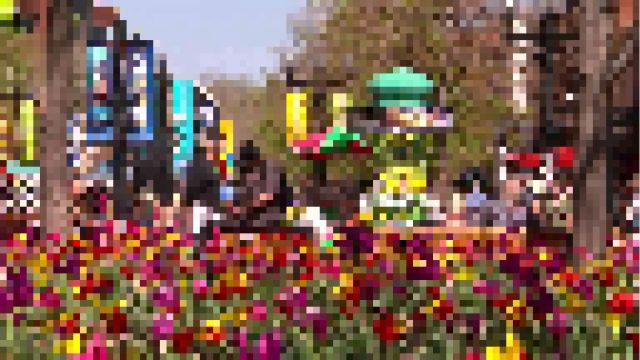
\includegraphics[ height=5cm, width=9cm]{blockiness}}
\caption{Przykładowy obraz z zakłóceniami spowodowanymi blokowością\cite{agh_vqm}}
\label{fig:xccs}
\end{figure}

\item Aktywność Przestrzenna ({\em ang. Spatial Activity}) -- opisuje położenie obiektu na ramce oraz jego relacje z innymi obiektami. Pozwala rozróżnić czy aktywność na danym wideo jest czynnością statyczną (osoba wykonująca czynność pozostaje w jednym miejscu) czy mobilną (osoba wykonująca czynność porusza się wzdłuż pola widzenia)\cite{spactial_act}. Skala przyjęta w pracy: 0-270. Im większa wartość tym większa aktywność przestrzenna\cite{agh_vqm}
\begin{center}
\centerline{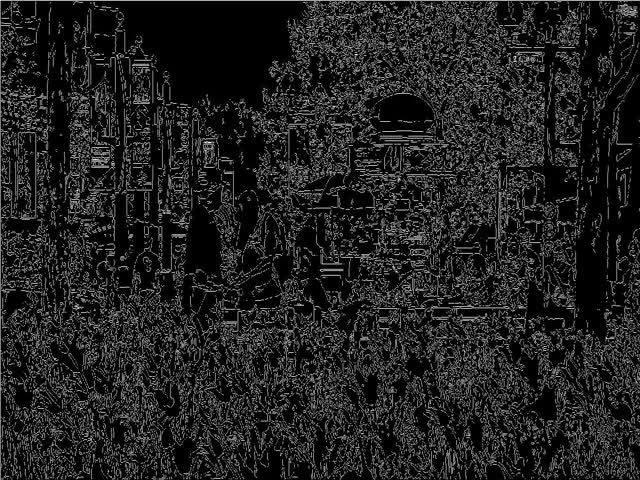
\includegraphics[ height=5cm, width=9cm]{spatialAC}}
\captionof{figure}{Przykład detekcji obiektów w ramce, niezbędne do otrzymania informacji o aktywnosci przestrzennej\cite{agh_vqm}}
\label{fig:xccs}
\end{center}


\item Letterbox i Pillarbox - letterbox jest techniką pozwalającą na wyświetlanie obrazów o wyższym współczynniku proporcji na odbiornikach o mniejszym współczynniku. Polega ona na dołożeniu dwóch czarnych pasów na górze i dole ramki.\cite{letterboxing}. Natomiast pillarbox używane jest przy wyświetlaniu obrazu w mniejszym współczynniku proporcji na ekranie o większym . Do obrazu dodawane są wtedy pasy po obu bokach ekranu. Skala przyjęta w pracy 0-1.
\begin{figure}[h]
\begin{subfigure}[b]{0.4\textwidth}
\centerline{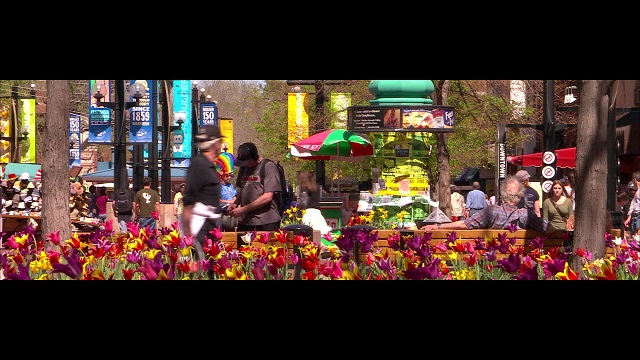
\includegraphics[ height=5cm, width=9cm]{letterboxingC}}
\caption{opis\cite{agh_vqm}}
\label{fig:xccs}
\end{subfigure} 
\hfill
\begin{subfigure}[b]{0.4\textwidth}
\centerline{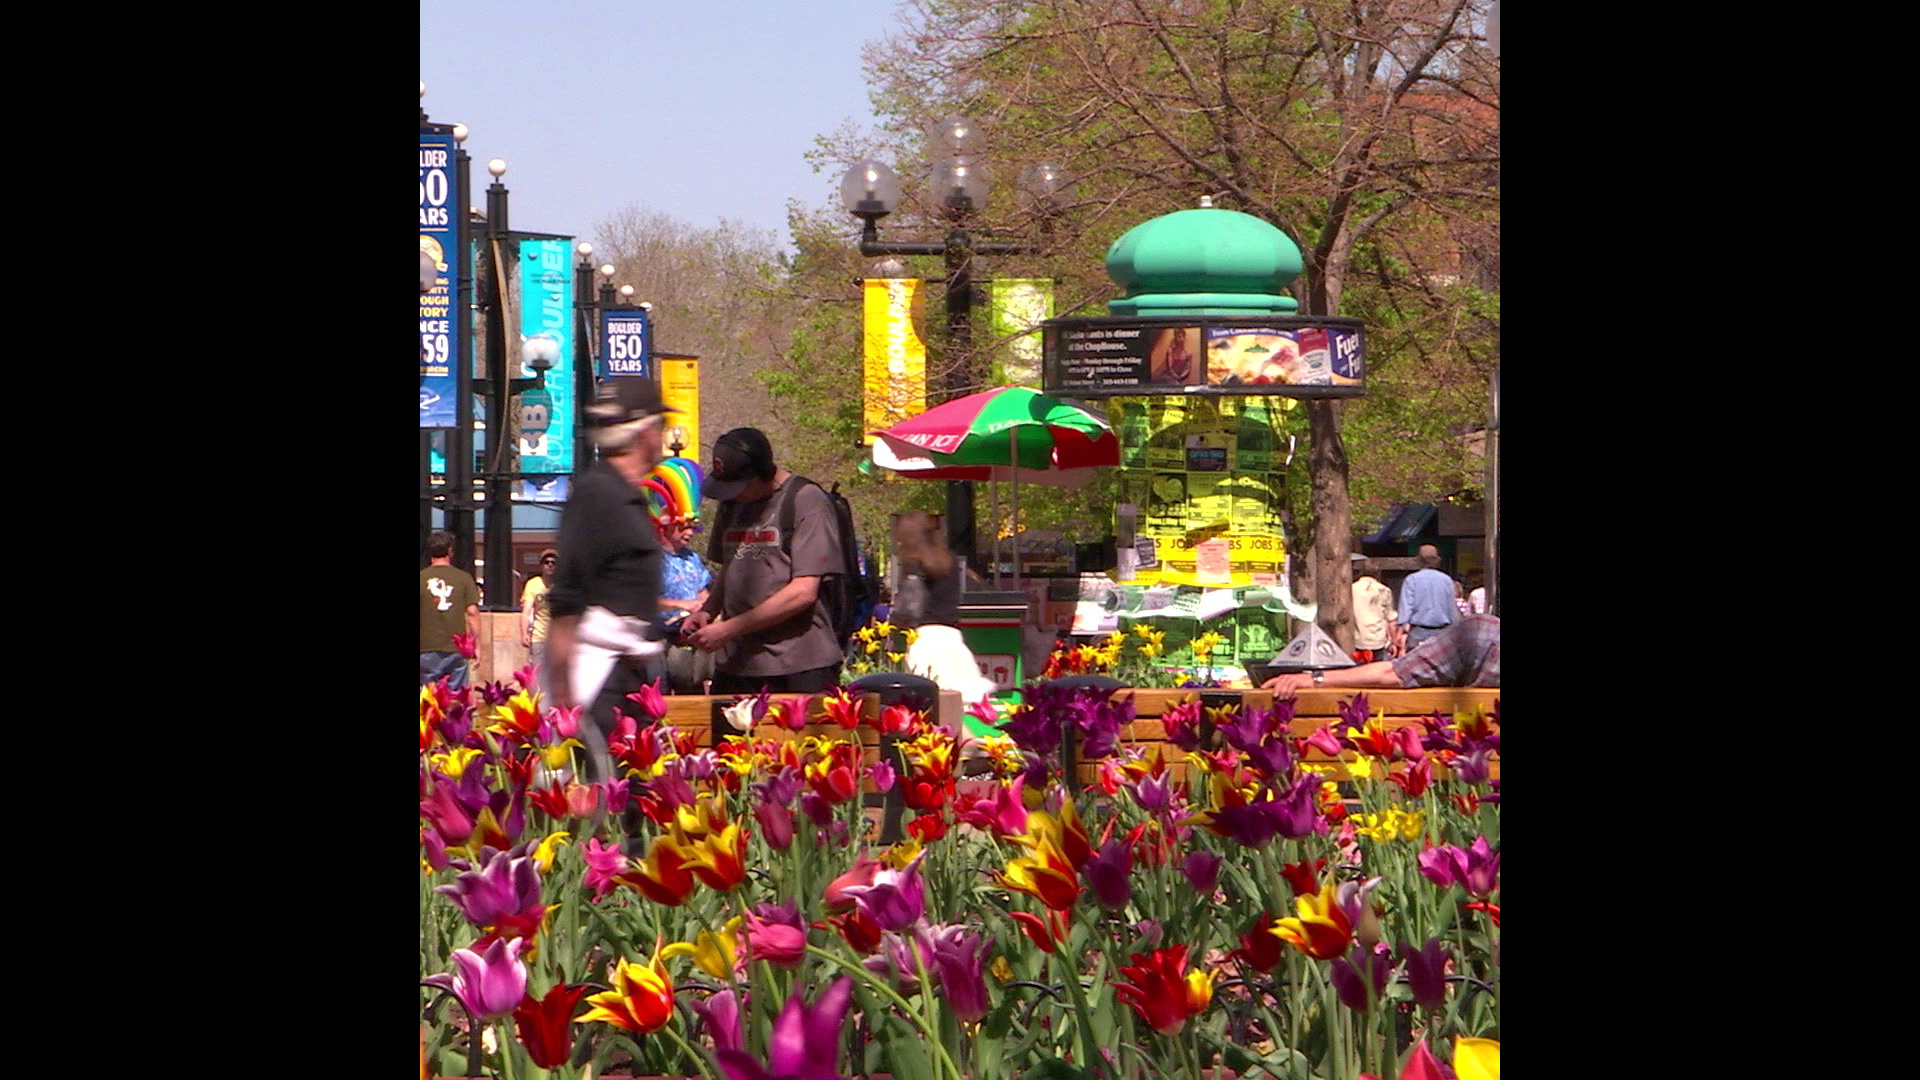
\includegraphics[ height=5cm, width=9cm]{pillarboxing}}
\caption{opis\cite{agh_vqm}}
\label{fig:xccs}
\end{subfigure}
\end{figure}

\item Straty bloków ({\em ang. Blockloss}) -- wskaźnik informujący o ilości brakujących bloków(używanych podczas DCT(Dyskretna transformacja kosinusowa)). Skala przyjęta w pracy: 0-200.Im większa wartość tym większe zniekształcenie obrazu.


\begin{center}
\centerline{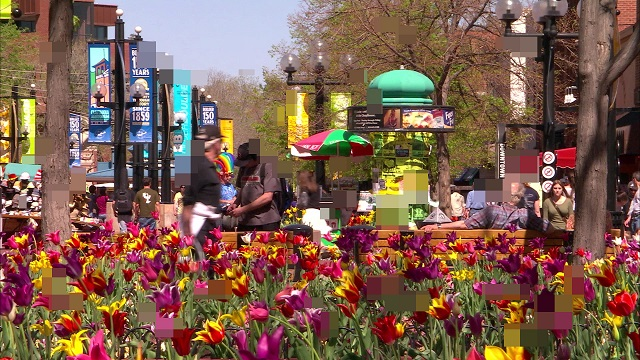
\includegraphics[ height=5cm, width=9cm]{block_lossC}}
\captionof{figure}{opis\cite{agh_vqm}}
\label{fig:xccs}
\end{center}

\item Rozmycie ({\em ang. Blur}) -- Istnieje wiele rodzajów rozmycia, między innymi te niepożądane, występujące po przeprowadzeniu kompresji bądź przez poruszenie kamerypodczas nagrywania. Gdy występuje ten efekt obiekty na obrazie tracą ostrość krawędzi.\cite{blur}. Skala przyjeta w pracy: 0-70.
\begin{center}

\includegraphics[ height=5cm, width=9cm]{blur}
\captionof{figure}{A non-floating figure \emph{with} a caption!}
\label{fig:xccs}
\end{center}

\item Aktywność czasowa ({\em ang. Temporal Activity}) -- opisuje intensywność ruchu obiektów w czasie. Często łączone ze wskaźnikiem aktywności przestrzennej. Skala przyjęta w pracy: 0-255.
\begin{center}
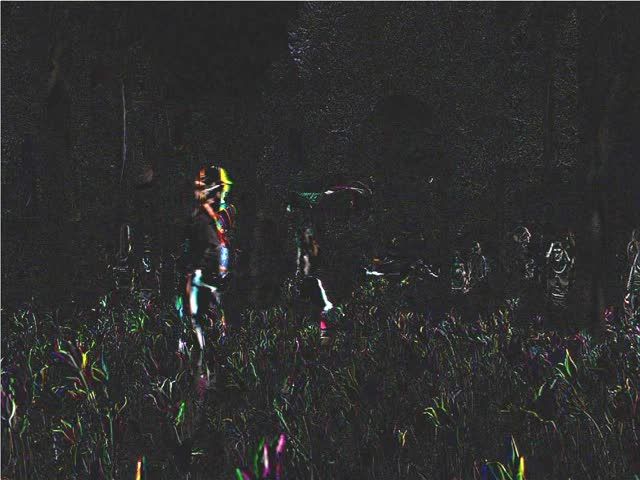
\includegraphics[ height=5cm, width=9cm]{temporalAC}
\captionof{figure}{A non-floating figure \emph{with} a caption!}
\label{fig:xccs}
\end{center}

\item Wyciemnienia ({\em ang. Blackout}) -- opisuje zjawisko, kiedy obraz całkowicie zanika\cite{blackout}. Skala przyjęta w pracy : 0-1
\begin{center}

\includegraphics[ height=5cm, width=9cm]{blackout}
\captionof{figure}{A non-floating figure \emph{with} a caption!}
\label{fig:xccs}elacpo
\end{center}

\item Zamrożenie ({\em ang. Freezing}) -- Informuje o efekcie czasowego zatrzymania zatrzymania obrazu, które powoduje odczucie "przycięcia" wideo\cite{freezing}. Skala przyjęta w pracy:0-1.

\item Ekspozycja ({\em ang. Exposure}) -- ten typ zakłóceń jest spowodowany niezbilansowaną jasnością ramek. Widz ma odczucie ze wideo jest zbyt ciemna lub zbyt jasne\cite{freezing}. Skala przyjęta w badaniach 0-255.
\begin{center}
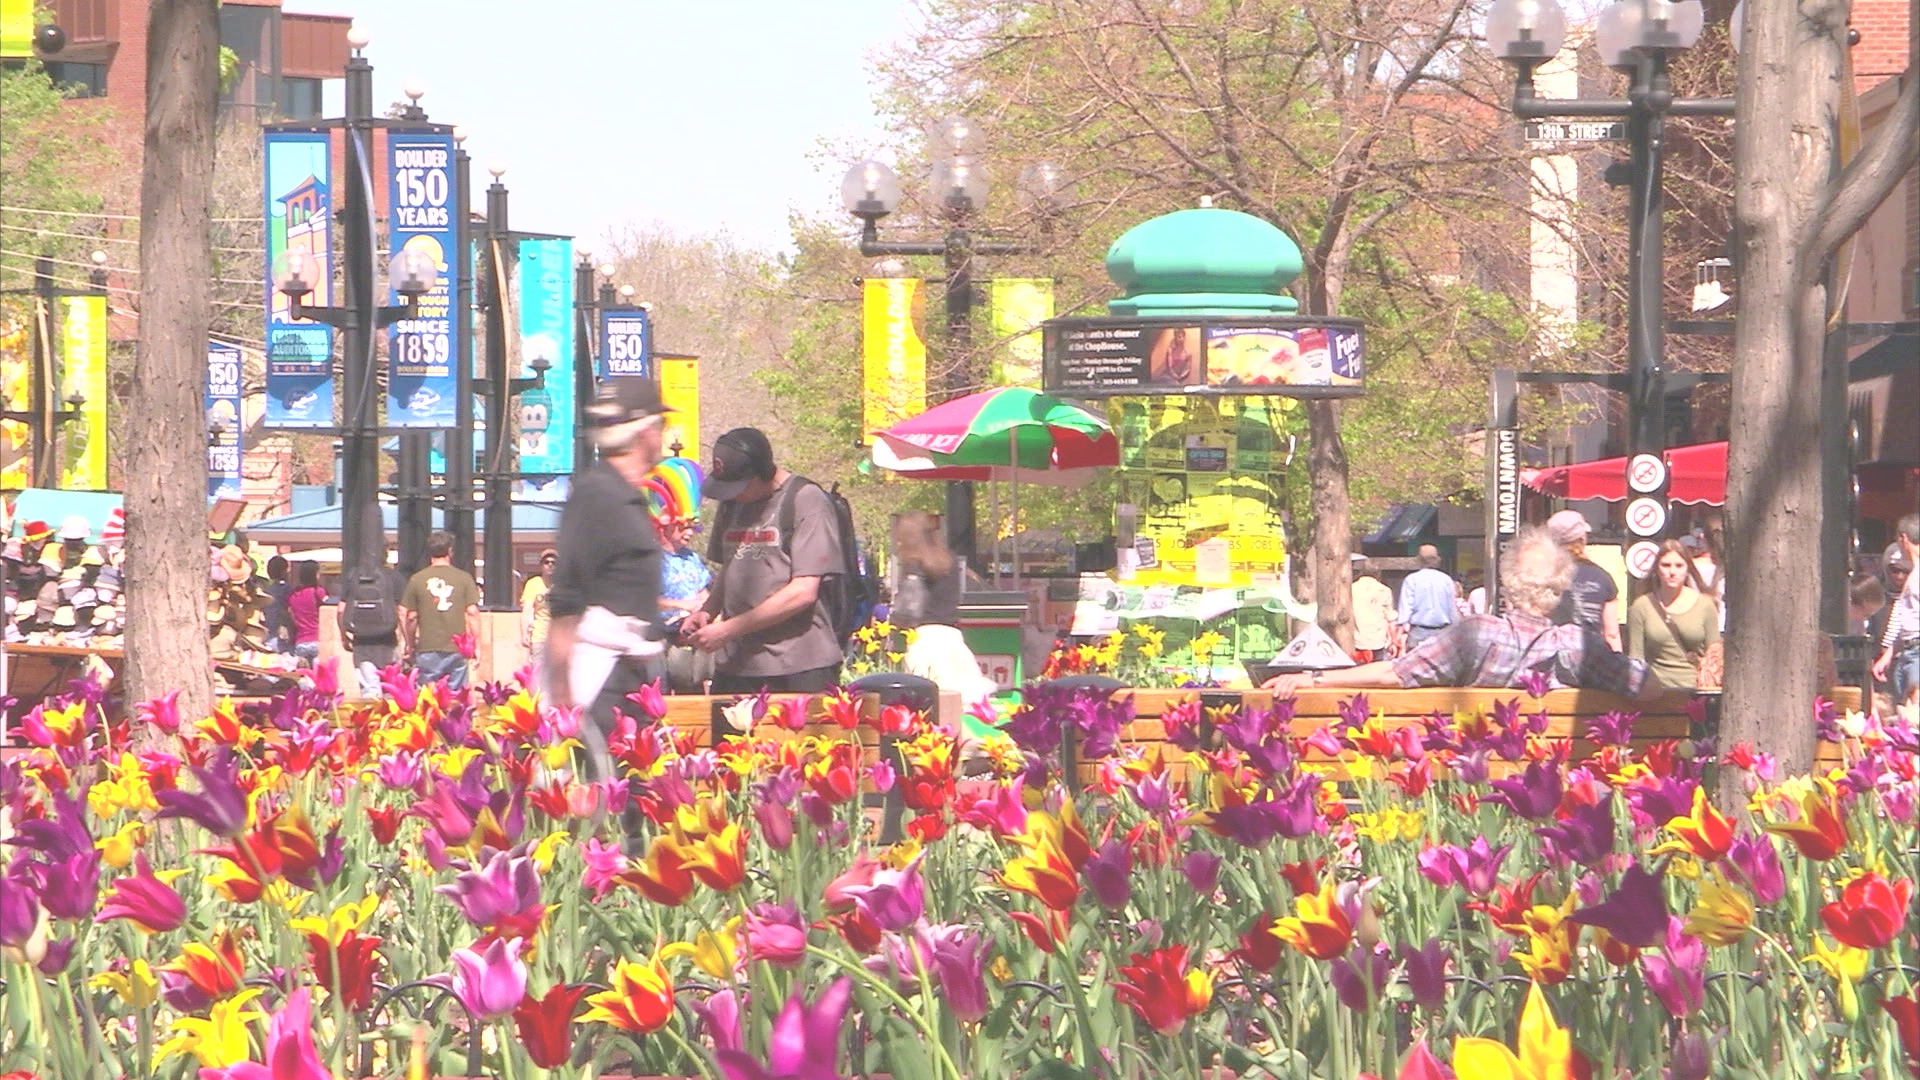
\includegraphics[ height=5cm, width=9cm]{exp}
\captionof{figure}{A non-floating figure \emph{with} a caption!}
\label{fig:xccs}
\end{center}


\item Kontrast ({\em ang. Contrast}) -- Opisuje różnice pomiędzy jasnymi, a ciemnymi obszarami obrazu. Skala przyjęta w pracy: 0-120.
\begin{center}
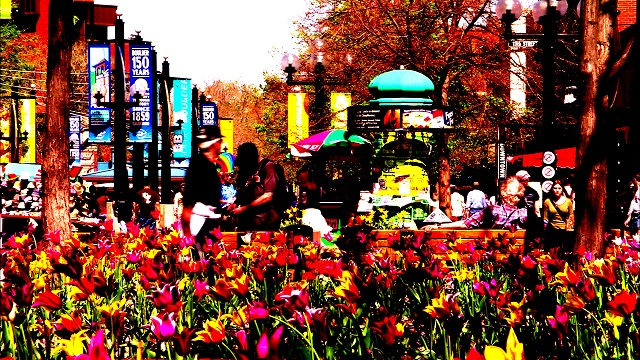
\includegraphics[ height=5cm, width=9cm]{contrastC}
\captionof{figure}{A non-floating figure \emph{with} a caption!}
\label{fig:xccs}
\end{center}
\item Jasnosć ({\em ang. Brightness}) -- jest powiązana z problemem Ekspozycji. Jej zbyt duża wartość może skutkować odczuciem przeswietlenia ramki. Skala przyjęta w pracy: 0-1.
\begin{center}
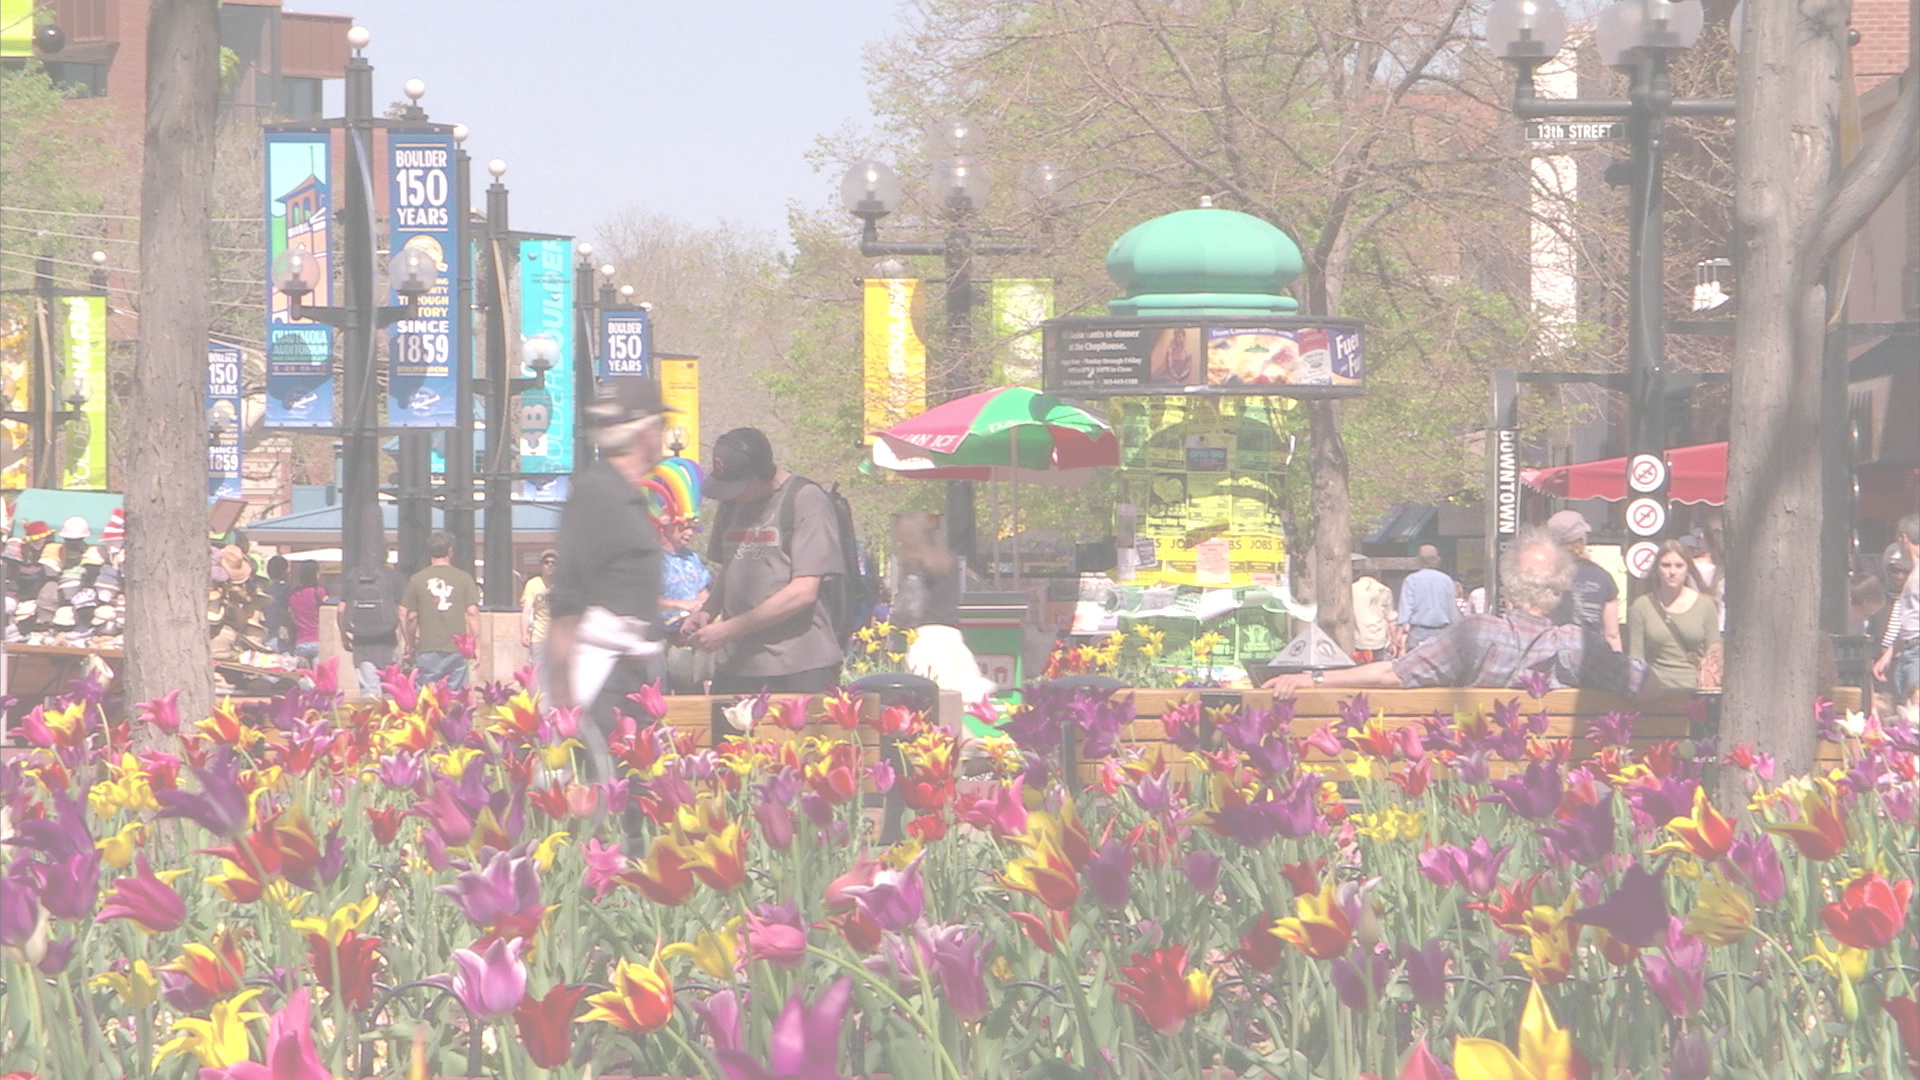
\includegraphics[ height=5cm, width=9cm]{brightness}
\captionof{figure}{A non-floating figure \emph{with} a caption!}
\label{fig:xccs}
\end{center}

%\item interlace Skala przyjęta w pracy: 0-1.
%\begin{figure}[h]
%\centerline{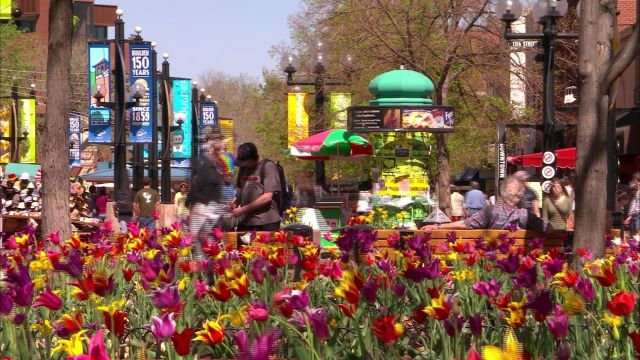
\includegraphics[ height=5cm, width=9cm]{interlace2C}}
%\caption{opis\cite{agh_vqm}}
%\label{fig:xccs}
%\end{figure}
\item Szum ({\em ang. noise}) -- jest to rodzaj zaburzenia obrazu spowodowany występowaniem niekontrolowanych wzorców dla intensywności wyświetlania pixeli\cite{freezing}. Skala przyjęta w pracy: 0-120.
\begin{center}
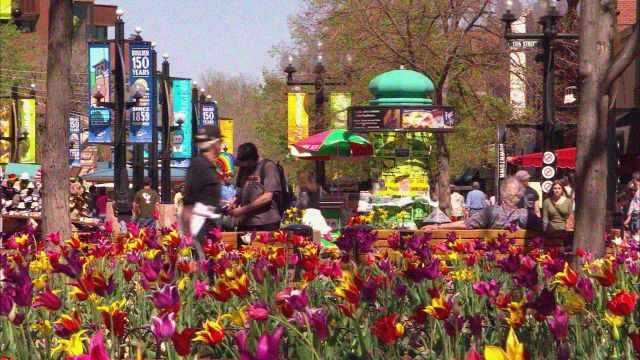
\includegraphics[ height=5cm, width=9cm]{noiseC}
\captionof{figure}{A non-floating figure \emph{with} a caption!}
\label{fig:xccs}
\end{center}
\item Pocięcie ({\em ang. Slice}) -- objawia się efektem niepasujących do całości poziomych pasów. Związane jest to utratą pakietów danych podczas transmisji wideo. NIE DZIALA POPRAWNIE ! 
\begin{center}
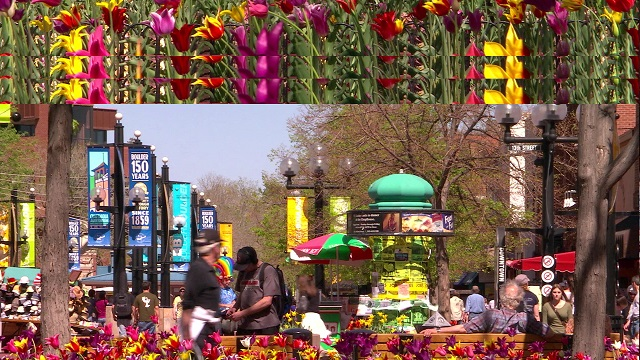
\includegraphics[ height=5cm, width=9cm]{slicingC}
\captionof{figure}{A non-floating figure \emph{with} a caption!}
\label{fig:xccs}
\end{center}
\end{itemize}
Oprócz wyżej wymienionych w pracy zostały również użyte dane o wideo taki jak: 

\begin{itemize}[label=$\bullet$]
\item Rozdzielczość ({\em Resolution}) -- miara określająca rozmiar ramki. Jednostką są pixele. Podawana jest zazwyczaj w następujący sposób: szerokość x wysokość. Do badań zostały użyto wideo o rozdzielczościach: 3840x2160, 1920x1080, 704x576, 640x480, 352x288. 
\item Klatki na sekundę ({\em ang. fps, frames per second}) -- liczba ramek wyświetlonych w czasie sekundy. W telewizji jest to 25 ramek na sekundę. Do badań użyto: 60, 30, 25, 24 fps
\item Kodowanie kolorów ({\em ang. Color encoding}) -- Jest to zabieg korzystający z niedoskonałoć ludzkiego oka i ma na celu zmiejszenie rozmiarów ramki. Dzieje się to po przez nie wysyłąnie informacji dotyczących kolorów, na każdego pixela. todo 
\end{itemize}


\subsection{Metryki full-reference}

\begin{itemize}[label=$\bullet$]
\item PSNR ({\em ang. Peak Signal-to-Noise Ratio}) -- prosta do policzenia i również często stosowane z pomiędzy metryk typu FR. Przykładowa implementacja dla PSNR \ref{eqn:somelabel} (gdzie MSE jest błędem średnio kwadratowym dla ramki). W pierwszej kolejności liczone jest zniekształcenie dla wszystkich ramek w stosunku do ich oryginału. Zazwyczaj do obliczań wykorzystuje się informację o luminacji pixela. Później następuje uśrednienie wyniku\cite{fr_psnr}. 
\begin{equation}
\label{eqn:somelabel}
PSNR = \frac{1}{N} \times 10 \sum_{i=1}^{N}\log\frac{255^2}{MSE_i}
\end{equation}
Mimo zalet PSNR nie zawsze spełnia swoje zadanie. Ilustracja \ref{fig:psnr_pict} przedstawia w różny sposób zniekształcone obrazy. Każdy z nich otrzymał tą samą ocenę PSNR, a jednak ocena subiektywna wskazuje na różny poziom jakości.
\begin{figure}[tbp]
\centerline{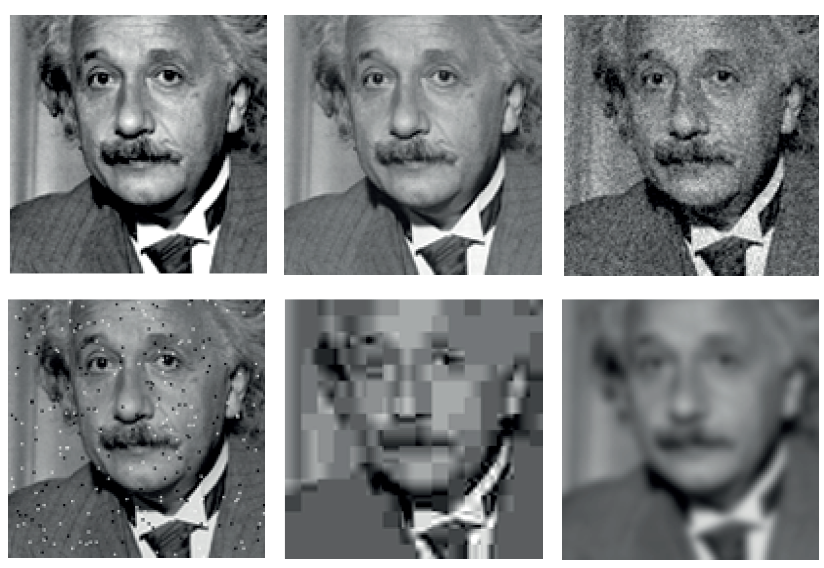
\includegraphics[ height=6cm, width=9cm]{psnr_pict}}
\caption{opis}
\label{fig:psnr_pict}
\label{fig:xccs}
\end{figure}

\item SSIM ({\em ang. Structural Similarity Index}) -- jest jedna z najczęściej stosowanych metryk oceny jakości wideo. Również, jak poprzednia metryka, jest ona prosta w obliczeniach. Uwzględnia w swojej funkcji luminacje, kontrast i strukturę obu \ref{eqn:ssim}, gdzie S jest blokiem pixeli z ramki z oryginalnej sekwencji wideo, a S' jej zniekształconą wersją. $SSIM \in <0,1>$. 1 oznacza brak zniekształceń, a 0 oznacza idealne niedopasowanie \cite{ssim_1}\cite{ssim_2}.
\begin{equation}
\label{eqn:ssim}
SSIM = I(S, S')c(S, S')s(S,S')
\end{equation}
\item MS-SSIM ({\em ang. multi-scale SSIM}) -- jest modyfikacją SSIM'a. Polega na próbkowaniu obrazu, w każdej skali, przed zastosowaniem SSIM'. Po przeprowadzeniu obliczeń, każda z skali jest łączona, z odpowiednimi wagami, w jedną całosć. Zabieg ma na celu poprawę trafności oceny jakości\cite{ssim_2}. 
\item VMAF ({\em ang. Video Multimethod Assessment Fusion}) -- Metryka rozwijana przez Netflix we współpracy z University of Southern California. Jej działanie opiera się na podłączaniu wyników kilku metryk podstawowych. VMAF nadaje każdej z metryk odpowiednie wagi ,a dzieje się to dzięki zastosowaniu algorytmu uczenia maszynowego, w tym przypadku SVM regressor ({\em ang. Support Vector Machine regressor}). Takie rozwiązanie ma zapewnić wykorzystanie mocnych stron poszczególnych metryk z pominięciem ich słabości \cite{netflix}. 
\end{itemize}

\section{Algorytmy uczenia maszynowego }

Obecne czasy charakteryzują się ogromną ilością danych, które zewsząd otaczają człowieka i jego środowisko. W każdej sekundzie różnego rodzaju dane są zbierane, przesyłane, prezentowane i analizowane. Aby móc, w optymalny sposób, czerpać z nich zyski zostały opracowane pewne algorytmy, bazujące na statystyce. Algorytmy te potrafią stworzyć modele matematyczne zadanego zdarzenia i na ich podstawie dokonać predykcji, klasyfikacji. Mogą również zinterpretować i zareagować na zadane sytuacje(?uczyc sie na swoich wlasnych obliczeniach?). Dziedzina nauki zajmująca się takimi algorytmami nazywana jest Uczeniem Maszynowym ({\em ang. Machine Learning}).\par
Wyróżniane są dwa typy algorytmów uczenia maszynowego: nadzorowane ({\em ang. supervised learning}) i nie nadzorowane({\em ang. unsupervised learning}). Różnica występuje podczas procesu tworzenia modelu -- trenowania. W pierwszej grupie, aby poprawnie zbudować model, wymagane jest aby dane treningowe składały się z par: dane wejściowe i oczekiwane dane wyjściowe(etykiety). Druga grupa nie wykorzystuję danych wyjściowych podczas trenowania. W badaniach zostały użyte algorytmy z uczeniem nadzorowanym, kolejne rozdziały będą odnosić się do tej właśnie grupy. Ponadto w pracy rozważany jest problem regresji, a więc dalsze opisy również będą się skupiać na tym aspekcie. \par
Głównym zadaniem algorytmów uczenia maszynowego jest odnalezienie jak najdokładniejszego przybliżenia funkcji: $f \colon X \to Y$. Jest to funkcja opisująca zależności pomiędzy danymi wejściowymi $X$, a danymi wyjściowymi $Y$\cite{ml_supervised}. Wskaźnik R-kwadrat($R^2$) pokazuje jak bardzo udało się zbliżyć do tej funkcji i definiowany jest wzorem \ref{eqn:r2}. 
\begin{equation}
\label{eqn:r2}
R^2=1- \frac{ \sum_{i=1}^{n}(Y_i-Y'_i)^2}{\sum_{i=1}^{n}(Y_i-\bar{Y}_i)^2 }
\end{equation}
$Y_i$ oznacza wartość szukanej przez model zmiennej, $Y'_i$ predykcję modelu, $\bar{Y_i}$ średnią wartość dla wszystkich $Y_i$. Przykładowo 1 oznacza idealne dopasowanie modelu, 0 oznacza ze model jest tak samo dokładny jak wartość średnia.\par
Poniższe podrozdziały zawierają krótki opis algorytmów użytych do badań w niniejszej pracy.



\subsection{Regresja Liniowa}
W Regresji Liniowej w jej podstawowej postaci zmienna niezależna $x_i$ ({\em ang. independent variable}) opisuje zamienną zależną $y_i$ ({\em ang. dependent variable}) zgodnie ze następującym wzorem $y_i = \beta_0 + \beta_1 x_i + \epsilon$. Gdzie $\beta_0$ i $\beta_1$ są współczynnikami określającym relację danych zmiennych $x$ i $y$. Do badań w pracy zostało wykorzystane pewne rozszerzenie klasycznej regresji liniowej, Wielokrotna Regresja Liniowa {\em ang. Multiple Linear Regression}, gdzie $y_i$ jest opisana następującą zależnością $y_i = \beta_0 + \beta_1 x_{1i} + \beta_2 x_{2i} + ... + \beta_p x+x_{pi} + \epsilon $ \cite{mlr}. Oznaczenia poszczególnych elementów tego równania są analogiczne do podstawowej wersji regresji. Trenowanie takiego modelu polega na szukaniu współczynników $\beta$.(?czy wpisywac cos o metodzie uczenia zaimplementowanej w skLearn, czyli :Ordinary Least Squares ?).\par

Regresja liniowa jest jednym z prostszych algorytmów. Jej cechą jest przejrzystość w interpretacji, dzięki możliwości zaobserwowania współczynników $\beta$. Regresja liniowa jest w stanie odnajdować zależności liniowe, natomiast dla zależności nieliniowych może dawać fałszywe wyniki.

\subsection{SVM}
{\em Software Vector Machine} (SVM) -- algorytm używany jako klasyfikator, który dokonuje podziału danych dzięki wcześniej wyznaczonej hiperpłaszczyźnie ({\em ang. hyperplane}). W celu zdefiniowania optymalnej hiperpłaszczyzny należy wyznaczyć maksymalną szerokość marginesów ({\em ang. margin} ) $\omega$, taką aby pojedyncze dane w różnych klas, znajdujące się najbliżej siebie, leżały na granicy marginesów. Takie dane definiowane są jako {\em ang. Support vectors}. Wielu przypadkach, aby podział danych był możliwy, należy użyć jednej z funkcji kernela, przenoszącej problem do więcej wymiarowej przestrzeni. Rysunek \ref{fig:svm} przedstawia przykładową hiperpłaszczyznę.\par
\begin{figure}[tbp]
\centerline{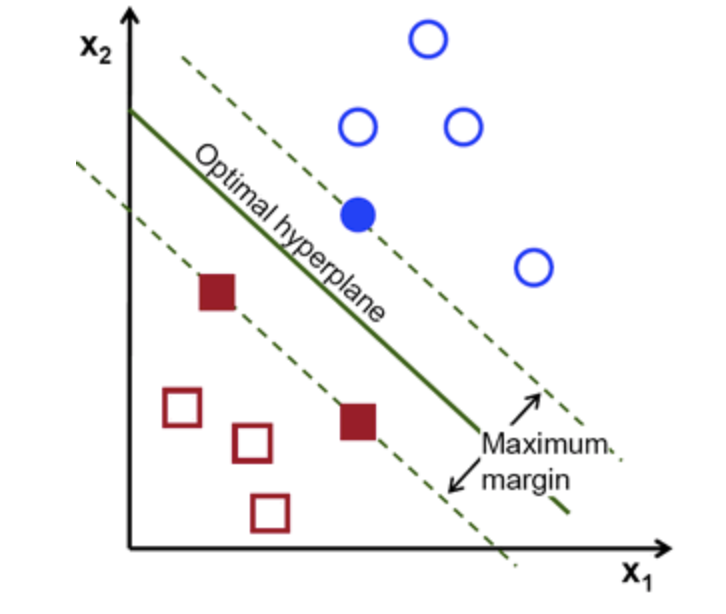
\includegraphics[ height=6cm, width=9cm]{svm}}
\caption{Hiperpłaszczyzna rozdzielająca dane, o dwóch właściwościach $x_1$ i $x_2$, na dwie klasy kół i kwadratów (obrazek mozna zmienic)}
\label{fig:svm}
\label{fig:xccs}
\end{figure}
W niniejszej pracy zostało użyte pewne rozwinięcie SVM, dla problemów dotyczących regresji, czyli SVR({\em ang. Support Vector Regression}). W takim rozwiązaniu hiperpłaszczyznę wyznacza się tak, aby jak najwięcej danych treningowych znalazło się w wybranej odległości $\epsilon$ od niej, w celu dopasowania funkcji $f \colon X \to Y$\cite{svr}. Zaletą SVM i SVR jest to, że są w stanie odnajdywać zależności nieliniowe, jednak by tego dokonać należy wybrać odpowiedną funkcję kernala, co często nie jest trywialne.

%SVR -> https://link.springer.com/chapter/10.1007/978-1-4302-5990-9_4
\subsection{Random Forest}
Random Forest działa w oparciu o "głosowanie"' wielu pojedynczy drzew. Każde z drzew powstaje dzięki implementacji algorytmu CART ({\em ang. Classification and Regression Trees}). W tym przypadku dla problemów regresji. Drzewa składają się z Węzła Głównego ({\em ang. Root Node}), Liści ({\em ang. Leaves}), Węzłów Decyzyjnych({\em ang. Decision Nodes}). Trenowanie drzewa bazuje na minimalizacji funkcji $S$ wyrażającej się wzorem \ref{eqn:rf}, gdzie $m_c=\frac{1}{n}\sum_{i \in c}y_i$ i jest predykcja z danego liścia\cite{rf}. Wizualizacja dopasowania funkcji na podstawie Drzewa Regresyjnego \ref{fig:r_tree}.\par
\begin{equation}
\label{eqn:rf}
S=\frac{1}{n}\sum_{c \in leaves(T)}\sum_{i \in c}(y_i - m_c)^2
\end{equation}
W Random Forest każde z drzew budowane jest w oparciu o inny podzestaw danych treningowych, co w swoim zamyśle ma na celu podwyższenie dokładności modelu oraz zmniejszenie zagrożenia nadmiernego dopasowania (ang. {\em overfitting})\cite{rf2}. Istotną kwestią jest dobór optymalnych parametrów dla modelu, takich jak liczba drzew oraz ich głębokość. 
\begin{figure}[tbp]
\centerline{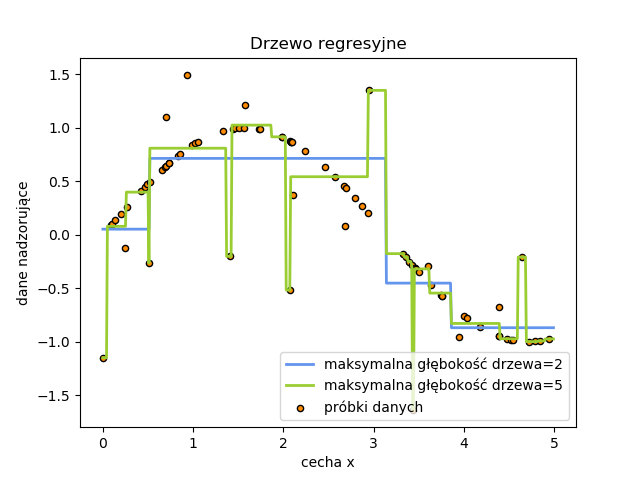
\includegraphics[ height=6cm, width=9cm]{r_tree}}
\caption{opis}
\label{fig:r_tree}
\label{fig:xccs}
\end{figure}

\subsection{Sieci Neuronowe}
Struktura Sieci Neuronowych ({\em ang. Neural Networks}) jest inspirowana budową mózgu. Jej podstawowym elementem są neurony, które formują warstwy, te z kolei dzielą się na warstwę wejściową, warstwę wyjściowa i warstwy ukryte. Rysunek \ref{fig:nn} przedstawia schemat przykładowej sieci neuronowej. Neurony jako dane wejściowe otrzymują dane wyjściowe, z odpowiednią wagą, z poprzednich neuronów. Neurony z warstwy wejściowej otrzymują przygotowane dane treningowe.\cite{rf2} Proces uczenia który ustawia wagi, a tym samym mów jak powinny wyglądać połączenia pomiędzy neuronami, nosi nazwę {\em Back Propagation}\cite{bp}.\par

Jedna z największych zalet Sieci Neuronowych jest to, że w porównaniu z innymi algorytmami uczenia maszynowego, w lepszym stopniu wykorzystuje duże ilości danych wejściowych\cite{nndata}. Zależność ta została zobrazowana na wykresie \ref{fig:nn_data}. Co więcej algorytm ten dobrze radzi sobie z zależnościami nieliniowymi. Minusem natomiast jest brak możliwości obserwacji jak algorytm doszedł do danego wyniku.
00097934
haykin.neural-networks.3ed.2009
%https://www.researchgate.net/publication/324728060_Lung_Cancer_Detection_using_Deep_Learning#pf18
\begin{figure}[tbp]
\centerline{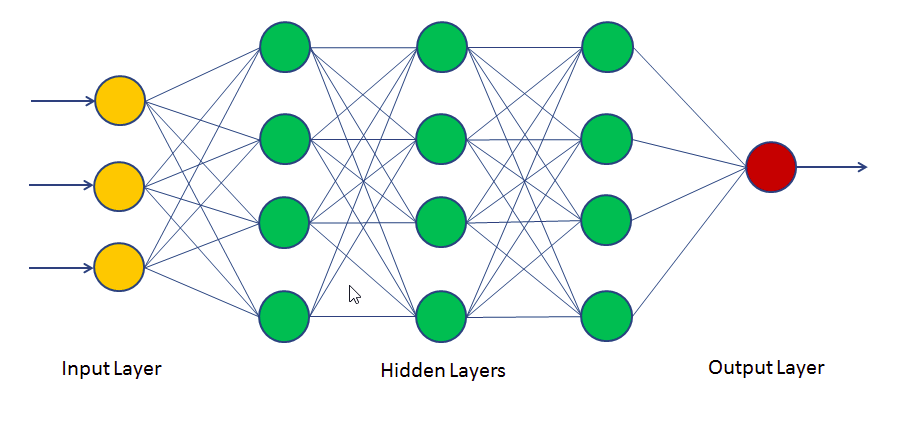
\includegraphics[ height=6cm, width=12cm]{nn}}
\caption{opis}
\label{fig:nn}
\label{fig:xccs}
\end{figure}

\begin{figure}[tbp]
\centerline{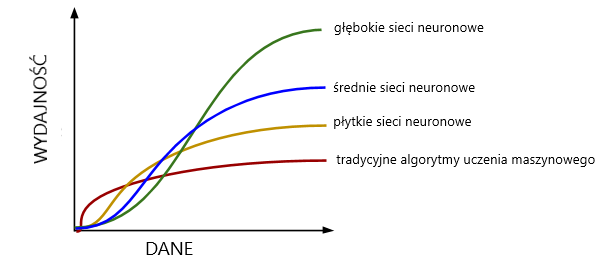
\includegraphics[ height=6cm, width=9cm]{nn_data_2}}
\caption{Wydajnosć Sieci neuronowych w porównaniu do tradycyjnych algorytmów uczenia maszynowego\cite{nn_wykres}.}
\label{fig:nn_data}
\label{fig:xccs}
\end{figure}


\chapter{Metodologia badań}
\label{cha:pierwszyDokument}

\section{Dane}
\label{cha:pierwszyDokument}

\begin{itemize}
\item Wybrane narzędzia
\item Opis zebranych danych
\item Przedstawienie data flow(pobieranie-> czyszczenie->normalizacja->przygotowanie formatu dla modeli).
\item Wizualizacja danych
\end{itemize}





\section{Modele }
\label{cha:pierwszyDokument}

\begin{itemize}
\item Opis zastosowanych parametrów/technik podczas trenowania.
\item Przedstawienie wyników 
\end{itemize}


\chapter{Analiza i wnioski }
\label{cha:pierwszyDokument}

\begin{itemize}
\item Interpretacja wyników
\item Opis innych czynników mogących zaburzyć ich prawdziwoć
\item Co nie zostało uwzględnione 
\end{itemize}


\chapter{Podsumowanie}
Zle nagranego wideo nie uratuje zadna metryka
Metryki powinny dostosowywac sie do (rodzaju zakłóceń)zaklocen
\label{cha:pierwszyDokument}

\begin{itemize}
\item Czy cel pracy został osiągniety.
\item Możliwoci rozbudowy
\end{itemize}








